[261~v\textsuperscript{o}] exiguas ipsi $\displaystyle L((H))$ aequales dividamus \edtext{rectam $\displaystyle LT$ et totum spatium quod a corpore per planum asperum decurrente ab initio ad finem motus usque percurritur, dividamus in totidem numero partes ipsius $\displaystyle LT$ partibus proportionales, ut si spatium quod a mobili ad quietem usque a frictione ortam percurretur sit [$\displaystyle D \aleph$]\edtext{}{\Bfootnote{$\displaystyle L \aleph$ \textit{\ L \"{a}ndert Hrsg.}}} et $\displaystyle DP$ sit ad $\displaystyle D \aleph$ ut $\displaystyle LV$ ad $\displaystyle LT$ tantum celeritatis perdet mobile percurrendo per $\displaystyle DP$, quantum 
acquireret descendendo per $\displaystyle LV$}{\lemma{rectam $\displaystyle LT$}\Bfootnote{\textit{(1)}\ tunc quantam \textit{(2)}\ et totum [...] planum \textbar\ asperum \textit{erg.}\ \textbar\ decurrente [...] proportionales, \textit{(a)}\ tunc portio quae \textit{(b)}\ ut si [...] perdet \textit{(aa)}\ $\displaystyle LV$ \textit{(bb)}\ mobile [...] per $\displaystyle LV$ \textit{L}}}[,]
ponendo $\displaystyle LV$ \edtext{esse altitudinem ad quam}{\lemma{esse}\Bfootnote{\textit{(1)}\ spatium ad quod grave\protect\index{Sachverzeichnis}{grave} \textit{(2)}\ altitudinem ad quam \textit{L}}} ascendere posset vi\protect\index{Sachverzeichnis}{vis} sua, initio frictionis, si motus \edtext{ejus sursum}{\lemma{ejus}\Bfootnote{\textit{(1)}\ libere \textit{(2)}\ sursum \textit{L}}} converteretur, nullaque frictio esset. Itaque uti sunt celeritates quaesitae in ratione spatii per quod descenditur, ita sunt celeritates perditae in ratione \edtext{spatii asperi}{\lemma{spatii}\Bfootnote{\textit{(1)}\ ad \textit{(2)}\ asperi \textit{L}}} quod percurritur.
Sunt autem corporibus 
descendentibus celeritates quaesitae in ratione \edtext{temporum insumtorum}{\lemma{temporum}\Bfootnote{\textit{(1)}\ percursorum \textit{(2)}\ insumtorum \textit{L}}}; seu in subduplicata ratione spatiorum percursorum; ergo et corporibus in plano aequaliter aspero percurrentibus erunt celeritates perditae in subduplicata ratione spatiorum \edtext{percursorum: Pone jam celeritatem primam fuisse $\displaystyle a$. spatium percursum esse $\displaystyle x$. celeritas perdita erit
$\displaystyle \sqrt{\protect\vphantom{2ax}}2ax$}{\lemma{percursorum:}\Bfootnote{\textit{(1)}\ Et tempora quoque insumta erunt in subduplicata ratione spatiorum percursorum. Aliter idem colligas, celeritates quaesitae \textit{(2)}\ Siv \textit{(3)}\ Pone [...] fuisse $\displaystyle a$. \textit{(a)}\ celeritatem perdit \textit{(b)}\ spatium [...] erit 
$\displaystyle \sqrt{\protect\vphantom{2ax}}2ax$
\textit{L}}}.
itaque celeritas residua
$\displaystyle a - \sqrt{2ax}$.
Jam temporum incrementa celeritatibus reciproca sunt. 
Ergo erunt
\rule[-4mm]{0mm}{10mm}$\displaystyle \frac{a^2}{a - \sqrt{\protect\vphantom{2ax}} 2ax} \sqcap \, y$.
Quaeritur summa ipsarum $\displaystyle y$ seu figurae ejusmodi quadratura, fiet:
$\displaystyle a^2 \sqcap \, ay - y \sqrt{\protect\vphantom{2ax}} 2ax$.
adeoque
$\displaystyle ay - a^2 \sqcap \, y \sqrt{\protect\vphantom{2ax}} 2ax$.
et quadrando:
\rule[-4mm]{0mm}{10mm}$\displaystyle \frac{a^2y^2 - 2a^3y + a^4}{2ay^2} \sqcap \, x$. adeoque
\rule[-4mm]{0mm}{10mm}$\displaystyle x \, \sqcap \, \frac{a}{2} - \frac{a^2}{y} + \frac{a^3}{2y^2}$.
Habetur \edtext{ergo hujus figurae quadratura}{\lemma{ergo}\Bfootnote{\textit{(1)}\ haec \textit{(2)}\ hujus figurae quadratura \textit{L}}} exposita quadratura Hyperbolae, adeoque etsi per ambitum, redit tamen ad
\pend
%\newpage
\count\Bfootins=1200
\pstart
\noindent Logarithmos. Itaque ex datis
     \edtext{temporibus insumtis spatia percursa, vel ex
    datis spatiis percursis insumta tempora definire}{\lemma{temporibus}\Bfootnote{\textit{(1)}\ spatia definire et \textit{(2)}\ percursis spatia insumta \textit{(3)}\ insumtis [...] definire \textit{L}}}\edtext{, opus est}{\lemma{definire,}\Bfootnote{\textit{(1)}\ res est quae \textit{(2)}\ opus est \textit{L}}} 
Logarithmis.
Nota \rule[-4mm]{0mm}{10mm}\edtext{si aequatio 
$\displaystyle \frac{a^2}{a - \sqrt{\protect\vphantom{2ax}}2ax} \sqcap y$
}{\lemma{si}\Bfootnote{\textit{(1)}\ quantitas 
$\displaystyle \frac{a^2}{a - \sqrt{\protect\vphantom{2ax}} 2ax}$
\textit{(2)}\ aequatio [...] $\displaystyle \sqcap \ y$ \textit{L}}}\edtext{ dividatur}{\lemma{$\displaystyle \sqcap \ y$}\Bfootnote{ \textit{(1) }\ multiplicetur \textit{ (2) }\ dividatur \textit{L}}} per 
$\displaystyle a + \sqrt{\protect\vphantom{2ax}}2ax$.
fiet:
\rule[-4mm]{0mm}{10mm}$\displaystyle \frac{a^2}{a^2 - 2ax} \, \sqcap \, \frac{y}{a + \sqrt{\protect\vphantom{2ax}}2ax}$.
et pro 
$\displaystyle a - 2x$ ponendo $\displaystyle z$.
fiet:
\rule[-4mm]{0mm}{10mm}$\displaystyle \frac{a}{z} \sqcap \frac{y}{a + \sqrt{a^2 - az}}$,
erit ergo figurae momentum ex vertice:
\rule[-4mm]{0mm}{10mm}\edtext{$\displaystyle a^2 + \sqrt{a^2 - az}$.
quod absolute haberi potest}
{\lemma{$\displaystyle a^2 + \sqrt{a^2 - az}$.}
\Bfootnote{\textit{(1)}\ quod pend \textit{(2)}\ quod [...] potest \textit{L}}}. 
Novus est hic modus ac notabilis transformandi formulas 
%\begin{wrapfigure}[8]{l}{0.3\textwidth}
%  \vspace*{-4mm}
%   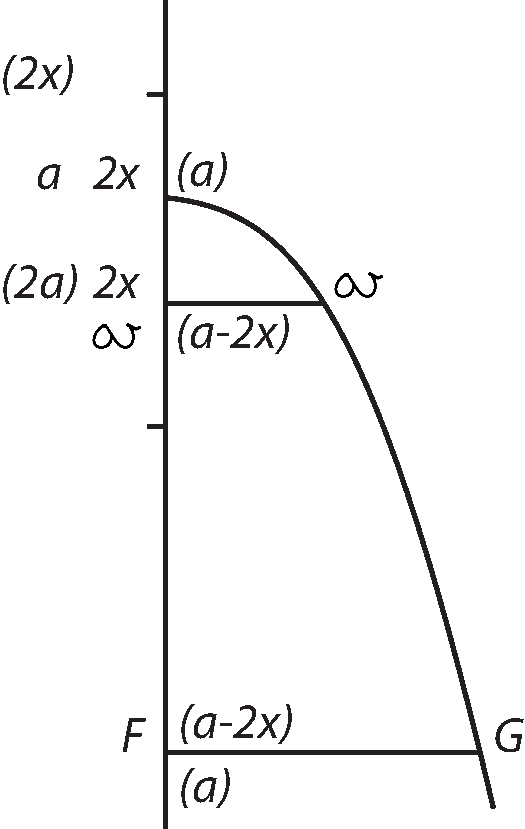
\includegraphics[trim = 0mm 0mm -10mm 0mm, clip, width=0.3\textwidth]{images/lh0351303_262r-d1.pdf}
%     \center[\textit{Fig. 2}] % \caption{Bildbeschreibung}
%    \end{wrapfigure} 
    curvarum: sed et 
\rule[-4mm]{0mm}{10mm}\edtext{$\displaystyle y \, \sqcap \frac{a^2 + a \sqrt{a^2 - az} + a^2 - az}{z}$
}{\lemma{$\displaystyle y \sqcap \frac{a^2 + a \sqrt{a^2 - az} + a^2 - az}{z}$}
\Cfootnote{Die Gleichung f\"{u}r $\displaystyle y$ widerspricht den vorausgegangenen Setzungen.}} 
sive 
$\displaystyle \frac{2a^2 -az + [a] \sqrt{a^2 - az}}{z}$,\edtext{}{\Bfootnote{$\displaystyle a$ \textit{\ erg. Hrsg.}}}
sive
\rule[-4mm]{0mm}{10mm}$\displaystyle y \, \sqcap \, \frac{2a^2}{z} - a + \frac{[a] \sqrt{a^2 - az}}{z}$.\edtext{}{\Bfootnote{$\displaystyle a$ \textit{\ erg. Hrsg.}}}\\
\hspace*{7,5mm}
Quaerendo ergo restat summa harum quantitatum 
\rule[-4mm]{0mm}{10mm}$\displaystyle \sqrt{\frac{a^2 - az}{z^2}}$ 
seu 
\rule[-4mm]{0mm}{10mm}$\displaystyle \frac{\sqrt{a^2 - az}}{z}$. 
Et fiet: 
\rule[-4mm]{0mm}{10mm}$\displaystyle \sqrt{\frac{a^2}{z^2} - \frac{a}{z}} \, \sqcap \, \frac{\omega}{a}$ sive $\displaystyle \frac{a^2}{z^2} - \frac{a}{z} + \frac{1}{4} \, \sqcap \, \frac{\omega ^2}{a^2} + \frac{1}{4}$ 
adeoque: 
\rule[-4mm]{0mm}{10mm}$\displaystyle\ \pleibdashv\displaystyle \frac{a}{z} \ \, \pleibvdash\displaystyle \frac{1}{2} \, \sqcap \, \frac{\sqrt{4\omega ^2 + a^2}}{2a}$, 
sive \rule[-4mm]{0mm}{10mm}$\displaystyle\ \pleibdashv\displaystyle [2]a^2\edtext{}{\Bfootnote{$\displaystyle 2$ \textit{\ erg. Hrsg.}}} \ \, \pleibvdash\displaystyle az \, \sqcap \, z \sqrt{4\omega ^2 + a^2}$
sive 
\rule[-4mm]{0mm}{10mm}$\displaystyle \frac{\efrac{}{\leibdashv} [2]a^2}{\, \efrac{}{\leibdashv} a + \sqrt{4\omega ^2 + a^2}}\edtext{}{\Bfootnote{$\displaystyle 2$ \textit{\ erg. Hrsg.}}} \, \sqcap \, z$\edtext{. quam proinde habere poterimus ex}{\lemma{\hspace{1.8mm}7--S. 328.1 \hspace{1.8mm}$\displaystyle \frac{\efrac{}{\leibdashv} [2]a^2}{\ \efrac{}{\leibdashv} a + \sqrt{4\omega ^2 + a^2}} \sqcap z$}\killnumber\Bfootnote{\textit{(1)}\ quae ideo etiam pendet ex quadratura hyperbolae \textit{(2)}\ quam [...] quadratura \textit{L}}}
\pend
\vspace{1.2em}
\pstart\centering
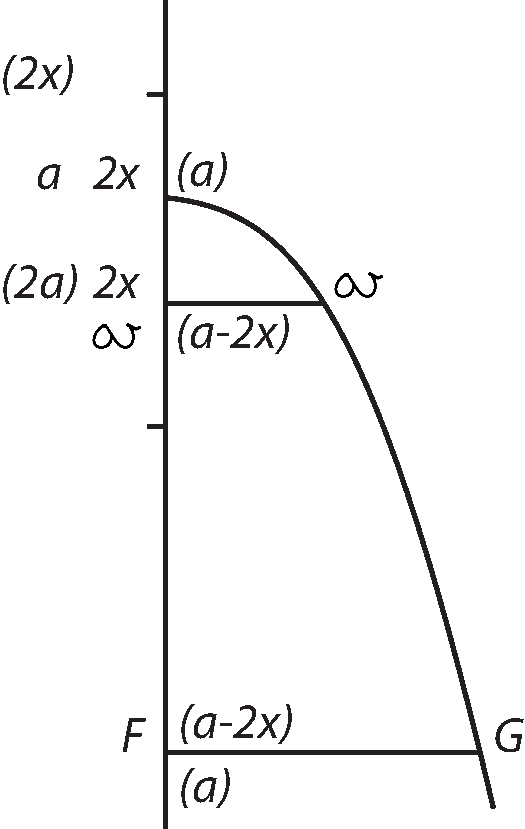
\includegraphics[trim = 0mm -3mm 0mm 0mm, clip, width=0.29\textwidth]{images/lh0351303_262r-d1.pdf}\\
     \centering [\textit{Fig. 2}] % \caption{Bildbeschreibung}
\pend
\newpage
\pstart\noindent
data hyperbolae quadratura.
%adeoque: 
%\rule[-4mm]{0mm}{10mm}$\displaystyle\ \leibdashv \frac{a}{z} \ \, \leibvdash \frac{1}{2} \, \sqcap \, \frac{\sqrt{4\omega ^2 + a^2}}{2a}$, 
%sive 
%\rule[-4mm]{0mm}{10mm}$\displaystyle\ \leibdashv [2]a^2 \ \, \leibvdash az \, \sqcap \, z \sqrt{4\omega ^2 + a^2}$\edtext{}{\Bfootnote{$\displaystyle 2$ \textit{\ erg. Hrsg.}}}
%sive 
%\rule[-4mm]{0mm}{10mm}$\displaystyle \frac{\leibdashv [2]a^2}{\, \leibdashv a + \sqrt{4\omega ^2 + a^2}} \, \sqcap \, z$\edtext{}{\Bfootnote{$\displaystyle 2$ \textit{\ erg. Hrsg.}}}\edtext{. quam proinde habere poterimus ex data hyperbolae quadratura}{\lemma{$\displaystyle \frac{\leibdashv [2]a^2}{\ \leibdashv a + \sqrt{4\omega ^2 + a^2}} \sqcap z$}\Bfootnote{\textit{(1)}\ quae ideo etiam pendet ex quadratura hyperbolae \textit{(2)}\ quam [...] quadratura \textit{L}}}.%\pend
